
\section{Motivation}
The energy efficiency of data centers has attained key importance in recent years, due to its high economic, environmental, and performance impact. 
Data center consumption was estimated in 2010 at between 1.1\% and 1.5\% of the worldwide electricity usage \cite{Dayarathna2016DataSurvey,Corcoran2017EmergingICT}, generating as much pollution as a nation like Argentina  \cite{Mathew2012Energy-awareNetworks}.
Power costs exceed in some cases the cost of purchasing hardware \cite{Rivoire2007ModelsOptimizations}. 
Nowadays, the leading petaflop supercomputers consume a range of 1-18 MW of electrical power, with 1.5 MW on average, which can be easily translated into millions of dollars per year in electricity bills \cite{Group2012HandbookSahni}.
Furthermore, the energy costs of powering a typical data center doubles every five years \cite{Buyya2013MasteringProgramming}.
Therefore, with such steep increase in electricity use and rising electricity costs, electricity bills have become a major expense for today's data centers \cite{Poess2008EnergyResults}, \cite{Gao2013QualityCenters}. 
Due to these reasons, data center energy efficiency is now considered a chief concern for data center operators, often ahead of the traditional considerations of availability and security.

There are several approaches for green computing, from electrical materials to circuit design, systems integration, and software. These techniques may be different, but they share the same goal: substantially reduce overall system energy consumption without a corresponding negative impact on delivered performance. 
%From a systems-software perspective, the strategy of supplying minimal power necessary to accomplish the work can be accomplished by powering down system components when they are underutilized \cite{Mathew2012Energy-awareNetworks}. 
From a software systems perspective, the strategy of providing just enough power to get a job done can be accomplished by turning off system components when they are underutilized \cite{Mathew2012Energy-awareNetworks}.
%The processor and main memory are usually in the top three power draw components, which dominate energy consumption as shown in figure \ref{fig:powerbreakdown}. 
The processor and main memory are usually the components that dominate power consumption, as shown in Figure  \ref{fig:powerbreakdown}.
The processor can consume as much as 50\% of the total energy \cite{Fan2007, Barroso2007TheComputing, Malladi2012TowardsDRAM}. For that reason, modern processors incorporate several features for power management \cite{Rotem2012Power-managementBridge, Brown2005, Hackenberg2015}, such as Dynamic Power Management (DPM) and Dynamic Voltage and Frequency Scaling (DVFS). 
DPM encompasses a set of techniques for obtaining an energy-efficient computing by deactivating or reducing the performance of system components when they are idle or used partially \cite{Shuja2012Energy-efficientCenters, Benini2000AManagement}.
DVFS allows the frequency and voltage to be adjusted in run-time depending on current needs.

\begin{figure}[ht]
	\centering
	\begin{subfigure}[b]{0.45\textwidth}
		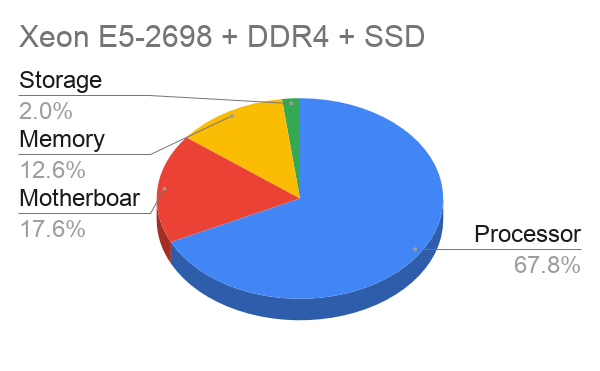
\includegraphics[width=\textwidth]{models/figures/power_breakdown/Xeon E5-2698 + DDR4 + SSD.png}
		\caption{This work}
		\label{fig:1}
	\end{subfigure}
	%
	\begin{subfigure}[b]{0.45\textwidth}
		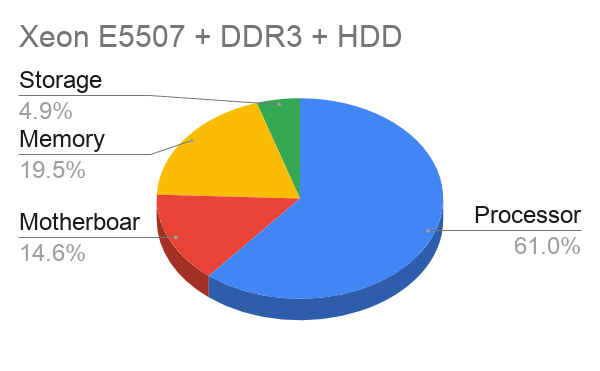
\includegraphics[width=\textwidth]{models/figures/power_breakdown/Xeon E5507 + DDR3 + HDD.png}
		\caption{Study case in \cite{Malladi2012TowardsDRAM}}
		\label{fig:2}
	\end{subfigure}
	
	\hfill
	\caption{Power breakdown of a typical node of an HPC cluster at full use. The system used in this work (a) was built in 2016 and equipped with two Intel Xeon E5-2698, 128 GB of DDR4 memory and SSD as storage, while (b) the case study in \cite{Malladi2012TowardsDRAM} was built in 2012 and equipped with two Xeon E5507, 32GB of DDR3 memory and HDD as storage}
	\label{fig:powerbreakdown}
\end{figure}

DVFS is motivated by the well-known fact that frequency and power have a near-cubic relationship \cite{Dayarathna2016DataSurvey, Group2012HandbookSahni}. 
This implies that running the CPU at lower frequency causes a linear reduction in the performance while a near-cubic reduction in power and, consequently, it could lead to a near-square reduction in CPU energy. 
This can lead to expressive energy savings depending on the system and its infrastructure.
Although very promising, the system software has yet to determine when and what voltage and frequency to use when running applications.
Otherwise, not only will performance deteriorate, but in the worst case, energy consumption would also increase  \cite{Group2012HandbookSahni}.
%Otherwise, in the worst case, not only performance will degrade, but also energy consumption may increase \cite{Group2012HandbookSahni}. 
Indeed, reducing the frequency results in a longer execution time, which in turn increases the energy consumption of other system components such as memory and disks.
%This is because reducing the frequency results in longer run time which in turn increases the energy consumption of the other components in the system such as memory and disks. 
There is also an overhead of time and energy associated with a voltage and frequency switch.
%There are also overheads of time and energy associated with a voltage and frequency switch.
Thus, finding the most appropriate voltage and frequency to use at all times is not an easy task.
%Finding the most appropriate voltage and frequency to use at each time instant is not an easy task. 
Therefore, since its introduction in 1994, there has been a lot of research on DVFS algorithms.
%Since its introduction in 1994, there has been a huge amount of work on DVFS algorithms in the literature.

The DPM technique can achieve very large energy savings on systems where the static power is high or when the system remains inactive for a long period.
In that case, the problem is to determine when and which components to turn on/off.
With DPM, energy savings of 70\% have been reported ~\cite{Shuja2012Energy-efficientCenters, Benini2000AManagement}.
%In the case of DPM, the problem is to determine when and which components to turn on/off. This technique can archive very large energy savings on systems where the static power consumption is high or if the system stays idle for a long time. Power savings of 70\% have been reported~\cite{Shuja2012Energy-efficientCenters, Benini2000AManagement}.

At the same time as the stated techniques reduce the energy consumption of the system, they also lead to a complex trade-off concerning performance, which must be exploited to produce more energy-efficient algorithms.
%However, at the same time that these power-saving techniques reduce system energy, they also lead to a complex balance between energy savings and high performance, exposing trade-offs between performance and power consumption, which can be exploited to produce more energy-efficient algorithms.  %in the case of the CPU, this can be applied to each core. Here... 
Indeed, this work investigates whether the construction of a model of the energy consumption of an application can lead to significant energy savings. We propose an analytical energy model of an application in function of the two control variables present in most of HPC systems: CPU operating frequency and number of active cores. This model can serve as a base for new DVFS and DPM algorithms, as well as for the analysis of the contribution of each model parameter to the total energy consumption. The model equation includes the two parameters of the application and three parameters of the system. The application parameters incorporate characteristics of the percentage of parallelism and the size of the input. The system parameters include power-related and technology-dependent components that compose dynamic, static and leakage power.

%The rest of this paper is divided as follows. In Section \ref{sec:relatedwork}, a general review of models is provided, showing the difference between each approach and its applications. In Section \ref{sec:models}, the models and its parameters are derived alongside its constraints. In section \ref{sec:experimentalvalidation}, the model is validated with the PARSEC benchmark applications. Forward, in Section \ref{sec:dvfs_optmin}, use cases of the model are presented, how it could be applied in DVFS and also analysis of the best saving energy policy depending on the system and the effect of the parallelism in the energy. Finally, the conclusion is make in Section \ref{sec:conclusion}.

%%%%%%%%%%%%%%%%%%%%%%%%%%%%%%%%%%%%%%%%%%

%\section{Related Work} \label{sec:relatedwork}
%
%A model is a formal abstraction of a real system. Models for computer systems can be represented as equations, graphical models, rules, decision trees, sets of representative examples, neural networks, etc. The choice of representation affects the accuracy of the models, as well as their interpretability by people \cite{Hypothesis2012EncyclopediaLearning}. Accurate energy and power consumption models are very important for many energy efficiency schemes employed in computing equipment \cite{Rivoire2007ModelsOptimizations} and they can have multiple uses, including the design, forecasting, and optimization of data center systems. This work focuses on analytical models that could serve for energy optimization and subsequently analysis of important factors in the total energy draw.
%
%The desirable properties of a full-system energy consumption model include accuracy (accurate enough to allow the desired energy saving), speed (generate predictions quickly enough), generality and portability (should be suitable for as many systems as possible), inexpensiveness (should not requires expensive or intrusive infrastructure), and simplicity \cite{Rivoire2008AModels}. However, modeling the exact energy consumption behavior of an HPC system is not straightforward, either at the whole-system level or at the individual component. Patterns of energy consumption in data centers depend on multiple factors such as hardware specifications, workload, cooling requirements, types of applications, etc. Some of these factors cannot be measured easily. Furthermore, it is impractical to perform detailed measurements of the energy consumption of lower-level components without introducing overhead to the system.
%
%The definition of energy (E) is the total amount of work performed by a system over a time period (T) while power (P) is the rate at which the work is performed by the system. The relationship between these three quantities can be expressed as:
%
%\begin{equation}
%E = \int_{0}^{T}P(t)dt
%\label{qe:energy_definition_cont}
%\end{equation}
%
%%Or in the discrete format, as the sum of energy in time windows $t_i$.
%
%%\begin{equation}
%%    E = \sum_{i}t_iP_i
%%    \label{qe:energy_definition_discrete}
%%\end{equation}
%
%As a starting point, the models were classified with respect to his inputs, based on the survey \cite{Dayarathna2016DataSurvey}, where they analyzed more than 200 models pointing their characteristics and limitations, it was possible to divide the models into the categories where is more suitable to drive their purposes.
%According to a survey over 200 models~\cite{Dayarathna2016DataSurvey} that analyzed their characteristics and limitations, they can be divided into categories that are are more suitable to drive their purpose:
%\begin{itemize}
%	\item Temperature
%	\item System Utilization or Workload
%	\item Frequency
%	\item Other system states such as: cache miss, branch prediction, number of instructions executed, and more
%	\label{tab:input_type}
%\end{itemize}
%
%%maybe split into power and performance models.
%Energy models are often described as a combination of two models, the power model of the system and the performance model of the application.
%
%\subsection{Power models}
%Temperature-based models can provide a way of estimating power consumption without being very intrusive. With this kind of model it is possible to estimate energy with a single temperature sensor without the need to restart or introduce anything to the system. This is especially interesting for HPCs and data centers which can not be easily turned off. Another use of this model is in optimization of the refrigeration systems.%, but this will be not covered in this journal.
%
%A large part of the developed models are based on system states. These types of models normally take advantage of performance counters, which are provided by the CPU or the operating system and are capable of counting micro-architectural events, such as: instructions executed, cache-hits, miss-predicted branches, and much more. This kind of model is great for power estimation because they have information about several internal states of the computer. It is possible to achieve accurate predictions within 2\% of error \cite{Joseph2001Run-timeMicroprocessors} in average. However, performance counters are highly dependent on the system and architecture, making them not so easily portable. Also, there are limitations on how many counters can be read simultaneously in the hardware side. The CPU only allows a small number of counters (normally five) to be read at the same time. If more counters are requested, some events will be multiplexed, causing measurement loss. From the software side, measuring a large number of system counters can introduce a significant overhead.
%
%Additionally, hardware performance counters had shown other problems \cite{Weaver2008, Weaver2013a, Das2019SoK:Security, McGuire2009, Ramos2019AnCounters}. Events that should be exact and deterministic (such as the number of executed instructions) show run-to-run variations and overcounting on x86\_64 machines, even when running in strictly controlled environments. Although this does not seem to be a problem when performing energy estimation---since normally the models have configurable weights or parameters that can account for imprecision, they might not be fully reliable.
%
%%include utilization
%
%Frequency-based models serve as base for many power models because at a very low level every digital circuit (including modern processors) is composed of transistors. In these devices, there is a known relationship between power and frequency, which can be simplified by equation \ref{eq:power_simplified}. 
%\begin{equation}
%P = \alpha+\beta f^3,
%\label{eq:power_simplified}
%\end{equation}
%where $\alpha$ and $\beta$ are model parameters and $f$ is the operating frequency. This equation is presented in more detail in Section~\ref{sec:models}.
%
%These models are good for the optimization problems since it is in function of a variable that can be easily controlled: $f$.
%%, although it is highly dependent on the load as shown in figure \ref{fig:cpuload}.
%
%% \begin{figure}
%%     \centering
%%     \includegraphics[width=0.5\columnwidth]{cpu_load.png}
%%     \caption{Power with a fixed frequency for different CPU loads, the load means the amount of time that the CPU was busy in the given time windows}
%%     \label{fig:cpuload}
%% \end{figure}
%
%Hybrid models can also be found in the literature. They are models that use as input frequency and CPU utilization or system states and frequency. In \cite{Horyath2008Multi-modeClusters}, they combine frequency and CPU utilization to obtain an average error of 1\% such as: 
%\begin{equation}
%P = a_3fu+a_2f+a_1u+a_0,
%\label{eq:hybrid}
%\end{equation}
%where $u$ is CPU utilization and $a_0$, $a_1$, $a_2$, $a_3$ are model parameters.
%
%\subsection{Performance models}
%Another very common way to model the energy consumption of the system is with the workload. The workload is an abstract definition of the application. It represents the amount of work done in a given time and speed \ref{eq:workload_definition}. Workload can be defined as~\cite{Paolillo2018OptimisationParallelism, Group2012HandbookSahni, Kim2015RacingHeuristics}:
%\begin{equation}
%W = \int_{0}^{T_{\rm active}}s(t)dt = sT_{\rm active},
%\label{eq:workload_definition}
%\end{equation}
%where $T_{\rm active}$ is total active time, and $s$ is the speed of execution. This kind of model is often translated into utilization-based models so that it is possible to work it in real systems. 
%% The definition of utilization is the ration of the time that the system was active. One possible transition is defined bellow in equation \ref{eq:workload_utilization_tranlation}.
%Utilization can be defined as the ratio between the time that the system is active and the total time. Equation \ref{eq:workload_utilization_tranlation} defines workload in terms of utilization.
%\begin{equation}
%u = \frac{T_{\rm active}}{T_{\rm total}} = \frac{w/s}{T_{\rm total}},
%\label{eq:utilization_definition}
%\end{equation}
%\begin{equation}
%w = usT_{\rm total}.
%\label{eq:workload_utilization_tranlation}
%\end{equation}
%
%Models based on CPU utilization are the bases for DVFS algorithms. Even though the input is not controllable, it is very easy to measure system utilization with almost no overhead. It is also very portable. There is no need for training and it often works reasonably in any machine. A downside is that the theory behind the energy consumption optimization relies on the knowledge of the future workload \cite{Fu2018RaceMinimization, Group2012HandbookSahni}. This introduces the problem of how to estimate the workload.
%
%%This models can be forward subdivided into  schedules, ...
%
%\subsection{Online vs Offline models}

\section{Theoretical background} \label{sec:background}

A model is a formal representation of a real system. Computer system models can be represented in the form of equations, graphical models, rules, decision trees, representative collections of examples, or by neural networks, among others. The choice of representation affects the model's accuracy, as well as its interpretability by people~\cite{Hypothesis2012EncyclopediaLearning, Roy2019ForecastingNetwork, Zhu2019PredictingLearning}. Accurate energy and power consumption models are very important for many energy efficiency schemes employed in computing equipment \cite{Rivoire2007ModelsOptimizations}, and they can have multiple uses, including the design, forecasting, and optimization of data center systems. This work focuses on analytical models that could serve for energy optimization and subsequently, analysis of important factors in the total energy draw.

The desirable properties of a full-system model of energy consumption include accuracy (precision enough to allow the required energy saving), speed (fast enough to produce predictions), generality and portability (should be suitable for as many systems as possible), inexpensiveness (should not require costly or invasive infrastructure), and simplicity \cite{Rivoire2008AModels}. However, modeling the exact energy consumption behavior of an HPC system is not straightforward, either at the whole-system level or at the level of individual components. Patterns of energy consumption in data centers depend on multiple factors such as hardware specifications, workload, cooling requirements, or types of applications. Some of these factors cannot be measured easily. Furthermore, it is impractical to perform detailed measurements of the energy consumption of lower-level components without impacting the system with additional overload.

The concept of energy (E) is the total amount of work performed by a system over a period of time (T), while power (P) is the rate at which the system performs the work. The relation between these three amounts can be expressed as:

\begin{equation}
E = \int_{0}^{T}P(t)dt
\label{qe:energy_definition_cont}
\end{equation}

Several proposed models have already been classified with respect to its input parameters in \cite{Dayarathna2016DataSurvey}. In this survey, more than 200 models were analyzed according to their characteristics and limitations and classified into categories where the model is more suited to its objectives:
\begin{itemize}
	\item Temperature
	\item System Utilization or Workload
	\item Frequency
	\item Other system states such as cache miss, branch prediction, number of instructions executed, and more
	\label{tab:input_type}
\end{itemize}

Often, energy models are described as a combination of two main parts, the power model of the system and the performance model of the application. 

\subsection{Power models}
Temperature-based models\cite{ZhangEnergyInfrastructure} can provide a way of estimating power consumption without being very intrusive. With this kind of model, it is possible to estimate energy with a single temperature sensor without the need to restart or introduce anything to the system. This is especially interesting for HPCs and data centers which, can not be easily turned off. Another use of this model is in the optimization of the refrigeration systems.

A large part of the developed models are based on parameters representing the state of the system. They normally take advantage of performance counters, which are provided by the CPU or the operating system and are capable of counting micro-architectural events, such as instructions executed, cache-hits, miss-predicted branches, and much more. 
This type of model is suitable for power estimation because it receives information about several internal states of the computer.

Frequency-based models serve as a base for many power models ~\cite{Sarwar1997, Butzen2007, Usman2013ANoC} because at a very low level every digital circuit (including modern processors) is composed of transistors. In these devices, there is a known relationship between power and frequency, which can be simplified by \cref{eq:power_simplified}: 
\begin{equation}
P = \alpha+\beta f^3
\label{eq:power_simplified}
\end{equation}
where $\alpha$ and $\beta$ are model parameters, and $f$ is the operating frequency (details of this equation are covered in Section~\ref{sec:models}). These types of models are suitable for optimization problems since they are a function of the operating frequency, which can be easily controlled.

\subsection{Performance models}
Another commonly used way to model the energy consumption of the system is the workload. The workload, which represents the amount of work done in a given time and speed, abstractly defines the application.  

The workload ($W$) can be defined as~\cite{Paolillo2018OptimisationParallelism, Group2012HandbookSahni, Kim2015RacingHeuristics}:
\begin{equation}
W = \int_{0}^{\tau}s(t)dt = s\tau
\label{eq:workload_definition}
\end{equation}
where $\tau$ is total active time, and $s$ is the execution speed in instructions/second.
This equation is often taken up by utilization-based models, so that it could be applied to real systems. 

Utilization can be defined as the ratio between the time that the system is active and the total time. Equation (\ref{eq:workload_utilization_tranlation}) defines workload in terms of CPU utilization ($u$):
\begin{equation}
u = \frac{\tau}{T} = \frac{W/s}{T},
\label{eq:utilization_definition}
\end{equation}
\begin{equation}
W = usT,
\label{eq:workload_utilization_tranlation}
\end{equation}
where $T$ the total execution time of the workload, and $s$ the execution speed.
Models based on CPU utilization are the base for DVFS algorithms. Even though the input is not controllable, it is straightforward  to measure system utilization with almost no overhead, and it is also very portable in terms of operating systems and architectures. 
%% Here is how to build the model or to optimize it, maybe too early to talk about AI without referencing existing approaches:
%There is no need for data and training, as with artificial intelligence algorithms, and adapts reasonably well to any machine. 
A downside is that optimization requires the knowledge of a wide variety of workloads which must be estimated somehow \cite{Fu2018RaceMinimization, Group2012HandbookSahni}.


% Markov model
Other approaches are also adopted to model energy, as for example in the work of Liu et al. \cite{Liu2016IntelligentSupplies} where the model uses a Markov chain to determine energy state transitions. This kind of approach needs heuristic algorithms to search for the best transitions and does not provide insights as an analytical equation does.

Although much work has been done in DVFS, the focus is still on the consumer electronics and laptop markets. 
For HPC, the notion of energy perception is relatively new~\cite{Beckman2005MakingSupercomputing}. 
Moreover, the operational characteristics of non-HPC and HPC systems are significantly different. 
First, the workload on non-HPC systems is very interactive with the end-user, but the workload on the HPC platform is not. 
Second, activities conducted on a non-HPC platform tend to share more machine resources.
In contrast, in HPC each job often runs with dedicated resources. 
Third, an HPC system usually is much larger than non-HPC systems, making it more  challenging to gather information, organize decisions, and execute global decisions.
Therefore, it is worthwhile to investigate whether a DVFS scheduling algorithm, which works well for conventional computing, remains effective for HPC.

\section{Related work} \label{sec:relatedwork}

Merkel et al.~\cite{Merkel2006BalancingSystems} developed an energy model for processors based on events. By counting a set of $n$ events and assuming that the processor consumes a fixed amount of energy $\alpha_i$ for each activity, they estimate the energy in a particular period as the number of occurrences $c_i$  multiplied by its correspondent weight $\alpha_i$:
\begin{equation}
E = \sum_{i=1}^{n}\alpha_ic_i.
\end{equation}

Another event-based model introduced by Roy et al. \cite{Roy2013AnAlgorithms}, described the computational energy consumed by a CPU for an algorithm $A$:
\begin{equation}
E(A) = P_{clk}T(A) + P_wW(A),
\end{equation}
where $P_{clk}$ is a processor clock leakage power, $T(A)$ is the total execution time, $W(A)$ is the total time taken by  non-I/O operations, and $P_w$ is used to capture the power consumption per operation performed by the CPU. $T(A)$ and $W(A)$ are estimated using performance features.

Models based on events are implemented using performance counters \cite{Fahad2019AComputing}, which have some drawbacks. They are highly dependent on the operating system and its architecture, making them not so easily portable. Additionally, there are limitations on the number of counters that can be read simultaneously. Furthermore, reading too many counters can add a non-negligible overhead. Thus, modern CPUs start to multiplex counters when more than a few are requested. There are also some well know problems regarding the precision of some events \cite{Weaver2008, Weaver2013a, Das2019SoK:Security, McGuire2009, Ramos2019AnCounters, Silva-De-Souza2020Containergy-aWorkloads}. Events that should be exact and deterministic (such as the number of executed instructions) show run-to-run variations and over-count on x86\_64 machines, even when running in strictly controlled environments. Our proposal is not based on performance counters and, therefore, is not vulnerable to those drawbacks.


Instruction-level energy model was also proposed in \cite{Characterization2013EnergyProcessor}, obtained from an energy per instruction (EPI) characterization made on Xeon Phi. Their model is expressed as:
\begin{equation}
E(f) = \frac{(p_1 - p_0)(c_1 - c_0)/f}{N}, 
\end{equation}
where $N$ is the total number of dynamic instructions, $p_0$ is the initial idle power, $p_1$ is the average dynamic power and ($c_1$-$c_0$) refers to the cumulative number of cycles the micro-benchmark performs. This model is suitable for estimating the energy after the application finishes executing, when it is possible to count the number of total cycles. However, it is challenging to use for optimization or forecasting since it does not have an application model to predict the number of cycles. Our model integrates the behavior of the application taking into account the execution time.

In \cite{Lewis2008Run-timeSystems} Lewis et al. described the overall system energy consumption using the following equation:
\begin{equation}
E = A_0(E_{proc} + E_{mem}) + A_1E_{em} + A_2E_{board} + A_3E_{hdd},    
\end{equation}
where, $A_0$, $A_1$, $A_2$, and $A_3$ are unknown constants that are calculated via linear regression analysis and those remain constant for a specific server architecture. This model, as the previous one, relies on knowledge of energy spent on each component, being  a suitable option for estimation after the application has already ran, but not for optimization of the run itself.

In another energy consumption model  based on system utilization, Mills et al. modeled the energy consumed by a compute node with CPU (single) executing at speed $\sigma$ as \cite{Mills2014EnergySystems},
\begin{equation}
E(\sigma,[t_1,t_2]) = \int_{t_1}^{t_2} \sigma^3 + \rho \sigma_max^3 dt,
\end{equation}

where $\rho$ stands for the overhead power  consumed regardless the processor speed, $t_1$ and $t_2$ are the initial and final execution time of the application. The overhead includes power consumption by all other system components such as memory, network, etc. For this reason, although the authors mentioned the energy consumption of a socket, their power model is generalized to the entire server.

Our work proposes a full-system energy model based on the CPU frequency and the number of cores.
The aim of the model is to understand and optimize the energy behavior of parallel applications in HPC systems according to application parameters such as the degree of parallelism and CPU parameters related to dynamic and static power. The proposed model differs from existing ones for including the frequency and number of cores in the same equation for estimating the energy for a specific application in a given configuration. This model can serve as a base for DVFS and DPM optimization problems that include frequency and number of active cores. It can also be used to analyze the contribution of each parameter (ex: level of parallelism) to energy consumption. The number of cores is an essential factor in HPC since applications are designed to run on multiple cores.

The proposed energy model is the product of an application-agnostic power model and an architecture-specific application performance model. The power model is based on the CMOS logic gates power draw as a function of the frequency~\cite{Sarwar1997, Butzen2007} augmented to include the number of cores. The performance model is based on Amdahl's law \cite{Amdahl1967ValidityCapabilities, Eyerman2010ModelingDesign, Shi2015ReevaluatingLaw}, which can be used to estimate runtime in multi-core systems. This model has been extended to include execution frequency and input size, characterizing the application on the target architecture.


\subsection{The contribution of this work}
Although a lot of work has been done in DVFS, the focus is still mainly on consumer electronics and laptop markets. For HPC, the notion of energy perception~\cite{Beckman2005MakingSupercomputing} is relatively new. Moreover, the operational characteristics of non-HPC and HPC systems are noticeably different. First, the workload on non-HPC systems is very interactive with the end-user, but the workload on the HPC platforms is not. Second, activities conducted on a non-HPC platform tend to share more resources of the machine. On the other hand, often in HPC, each job runs with dedicated resources. Third, an HPC system is normally much larger than non-HPC systems, which makes collecting information, organizing decisions, and executing global decisions more challenging. Therefore, it is worthwhile to investigate whether a DVFS scheduling algorithm, which works well for conventional computing, remains effective for HPC.

This work proposes a full-system energy model based on the CPU frequency and the number of cores. The goal of the model is to understand and optimize the energy behavior of parallel applications in HPC systems according to the application parameters such as the degree of parallelism and CPU parameters that relates to dynamic and static power. The proposed model differs from existing ones for including the frequency and number of cores in the same equation for estimating the energy for a specific application in a given configuration. This model can serve as a base for DVFS and DPM optimization problems that include both frequency and number of active cores. It can also be used to analyze the contribution of each parameter (ex: level of parallelism) to the energy consumption. The number of cores an important factor in HPC since applications are designed to run on multiple cores.

The proposed energy model is the product of an application-agnostic power model and an architecture-specific application performance model. The power model is based on the CMOS logic gate power draw in the function of the frequency~\cite{Sarwar1997, Butzen2007} augmented to include the number of cores. The performance model is based on Amdahl's law \cite{Amdahl1967ValidityCapabilities, Eyerman2010ModelingDesign, Shi2015ReevaluatingLaw}, which can be used to estimate execution time in multi-core systems. We have extended  this model to include the frequency and input size, characterizing the application on the target architecture.

%%%%%%%%%%%%%%%%%%%%%%%%%%%%%%%%%%%%%%%%%%

%\subsection{Goals of the research}
%
%The interest in developing this project is to make HPC increasingly viable, in addition to reducing maintenance costs and reducing the impact on the environment by saving energy.
%
%Apart from this, our research also has international collaborations with other high-performance computing centers such as the Federal University of Rio Grande do Norte, where the project was started, and others which I had collaborated with projects related to energy saving in the University of Bristol, and possible future collaborations with University of Lausanne on Switzerland.
%
%The main contribution of this thesis will be to produce better energy saving techniques for HPC based on dynamic models of applications’ performance, power/energy consumption analysis and extended DVFS techniques. As will be detailed in the next section, several objectives have been defined to address the multiple challenges of our proposal: consideration of the processor workload, instruction set and the input size of applications, more precise energy models based on additional execution parameters, alternative optimization strategies and automatization of the execution process.
%
%First experiments developed showed that this methodology has a potential and can be improved to develop software as an end product that can be used by servers and clouds to save energy. This search can also be easily expanded to encompass mobile devices such as smartphones or microprocessed devices like raspberry-pi and beaglebone. Contributions in the areas of power consumption modeling and algorithms for frequency and voltage control off the processor are the product of this research.
%
%\subsection{Work plan}
%
%Important points that will be addressed in this research:
%\begin{enumerate}
%	\item \textbf{Identify and analyzing important performance features for energy consumption}. Analyzing the application execution with multiple inputs on different configurations of active cores and frequencies, performance parameters and its relations can be chosen and associated to characterize the application. Since there is a large number of performance parameters, a study to select the principal components is necessary to reduce its complexity. 
%	\item \textbf{Splitting the application into optimizable execution steps}. The goal is to split the application execution into several stages and minimize the energy on each stage, for that, the performance model is going to be completely remodeled. Creating a complete profile of the application, including performance parameters, frequency, and a number of active cores. With this, we can Cluster the applications identifying common frequency scaling stages to optimize. So when the application is running we can collect these performance features and find the closest cluster that will already have the optimized configuration.
%	\item \textbf{Enhanced power models for HPC architectures: The power model is going to include additional parameters, such as the percentage of CPU utilization}. Further analysis of additional parameters, such as the influence of the instructions to be executed on the power consumed. Developing models that can reduce the overhead of training fitting and use fewer samples.
%	\item \textbf{Enhanced DVFS models for HPC architectures: Including new architectures with distributed memory and heterogeneous systems}. Also studied the viability of using mathematical and artificial intelligence models, their advantages and their trade-offs to produce the final model. With these tools develops we can extend the current DVFS algorithms and produce a Smart DVFS module for HPC.
%\end{enumerate}
%
%The new workflow that we want to implement can be illustrated on the figures \ref{fig:new_model} and \ref{fig:heterogeneous_systems}.
%
%\begin{figure}[h]
%	\centering
%	\includegraphics[width=\columnwidth]{intro/figures/new_model.png}
%	\caption{New model}
%	\label{fig:new_model}
%\end{figure}
%
%\begin{figure}[h]
%	\centering
%	\includegraphics[width=\columnwidth]{intro/figures/heterogeneous_systems.png}
%	\caption{Heterogeneous systems}
%	\label{fig:heterogeneous_systems}
%\end{figure}

